\documentclass[12pt]{beamer}

%  CORE PACKAGES --------------------------------
\usepackage{amsmath, amssymb, graphicx, booktabs, tabularx, setspace, soul}
\usepackage{subcaption}
\usepackage{tikz, pgfplots}
\pgfplotsset{compat=1.18}
\usetikzlibrary{positioning, arrows.meta, arrows.meta, positioning, shapes, calc}
\usepackage[many]{tcolorbox}
\usepackage[ruled,vlined]{algorithm2e}
\usepackage{minted}

%  FONTS & STYLING ------------------------------
\usepackage{fontspec}
\usefonttheme{professionalfonts}
\setsansfont[
UprightFont     = *Light,
BoldFont        = *Bold,
ItalicFont      = *Light Italic,
BoldItalicFont  = *Bold Italic,
Ligatures       = TeX,
Scale           = MatchLowercase
]{Frutiger LT Pro}
\renewcommand{\familydefault}{\sfdefault}
\linespread{1.}\selectfont
\hyphenpenalty=10000
\exhyphenpenalty=10000

%  COLORS & THEMES ------------------------------
\definecolor{aggiemaroon}{RGB}{80,0,0}
\definecolor{beamer@blendedblue}{RGB}{80,0,0}
\usecolortheme{default}

\setbeamertemplate{itemize items}{•}
\setbeamertemplate{itemize subitem}[•]
\setbeamertemplate{itemize subsubitem}[•]
\renewcommand{\UrlFont}{\ttfamily\small}

%  HYPERLINKS -----------------------------------
\usepackage{hyperref}
\hypersetup{
colorlinks=true,
linkcolor=aggiemaroon,
urlcolor=aggiemaroon,
citecolor=aggiemaroon
}

%  BEAMER TEMPLATES -----------------------------
\setbeamertemplate{caption}[numbered]
\setbeamertemplate{navigation symbols}{}
\setbeamertemplate{footline}{
\color{aggiemaroon}{\hfill \insertframenumber/\inserttotalframenumber \hspace{2pt} \vskip2pt}
}

%  CUSTOM ENVIRONMENTS --------------------------
\newenvironment{stepenumerate}{
\begin{enumerate}[<+->]
}{\end{enumerate}}

\newenvironment{stepitemize}{
\begin{itemize}[<+->]
}{\end{itemize}}

\newenvironment{stepenumeratewithalert}{
\begin{enumerate}[<+-| alert@+>]
}{\end{enumerate}}

\newenvironment{stepitemizewithalert}{
\begin{itemize}[<+-| alert@+>]
}{\end{itemize}}

% DOCUMENT INFO ---------------------------------
\title{Decision and Risk Analysis}
\subtitle{\textbf{Introduction}}
\author{\emph{}}
\date{\color{aggiemaroon}{
DAEN 427/ISEN 427/ISEN 627\\
\textbf{Alexander Abuabara}\\
Fall 2026
}}
\titlegraphic{\vfill 
\includegraphics[height=1.2cm]{TAMU_logo.png}}

% -----------------------------------------------
\begin{document}

% -----------------------------------------------
\maketitle

% -----------------------------------------------
\begin{frame}{}
\begin{block}{\emph{Yo, I'll tell you what I want, what I really really want}$^*$}
\begin{itemize}
    \item To be a great teacher and that means always learning, adapting, and getting better each and every day.
    \item That you learn concepts, analyze data, pass the class!
\end{itemize}
\end{block}
\centering
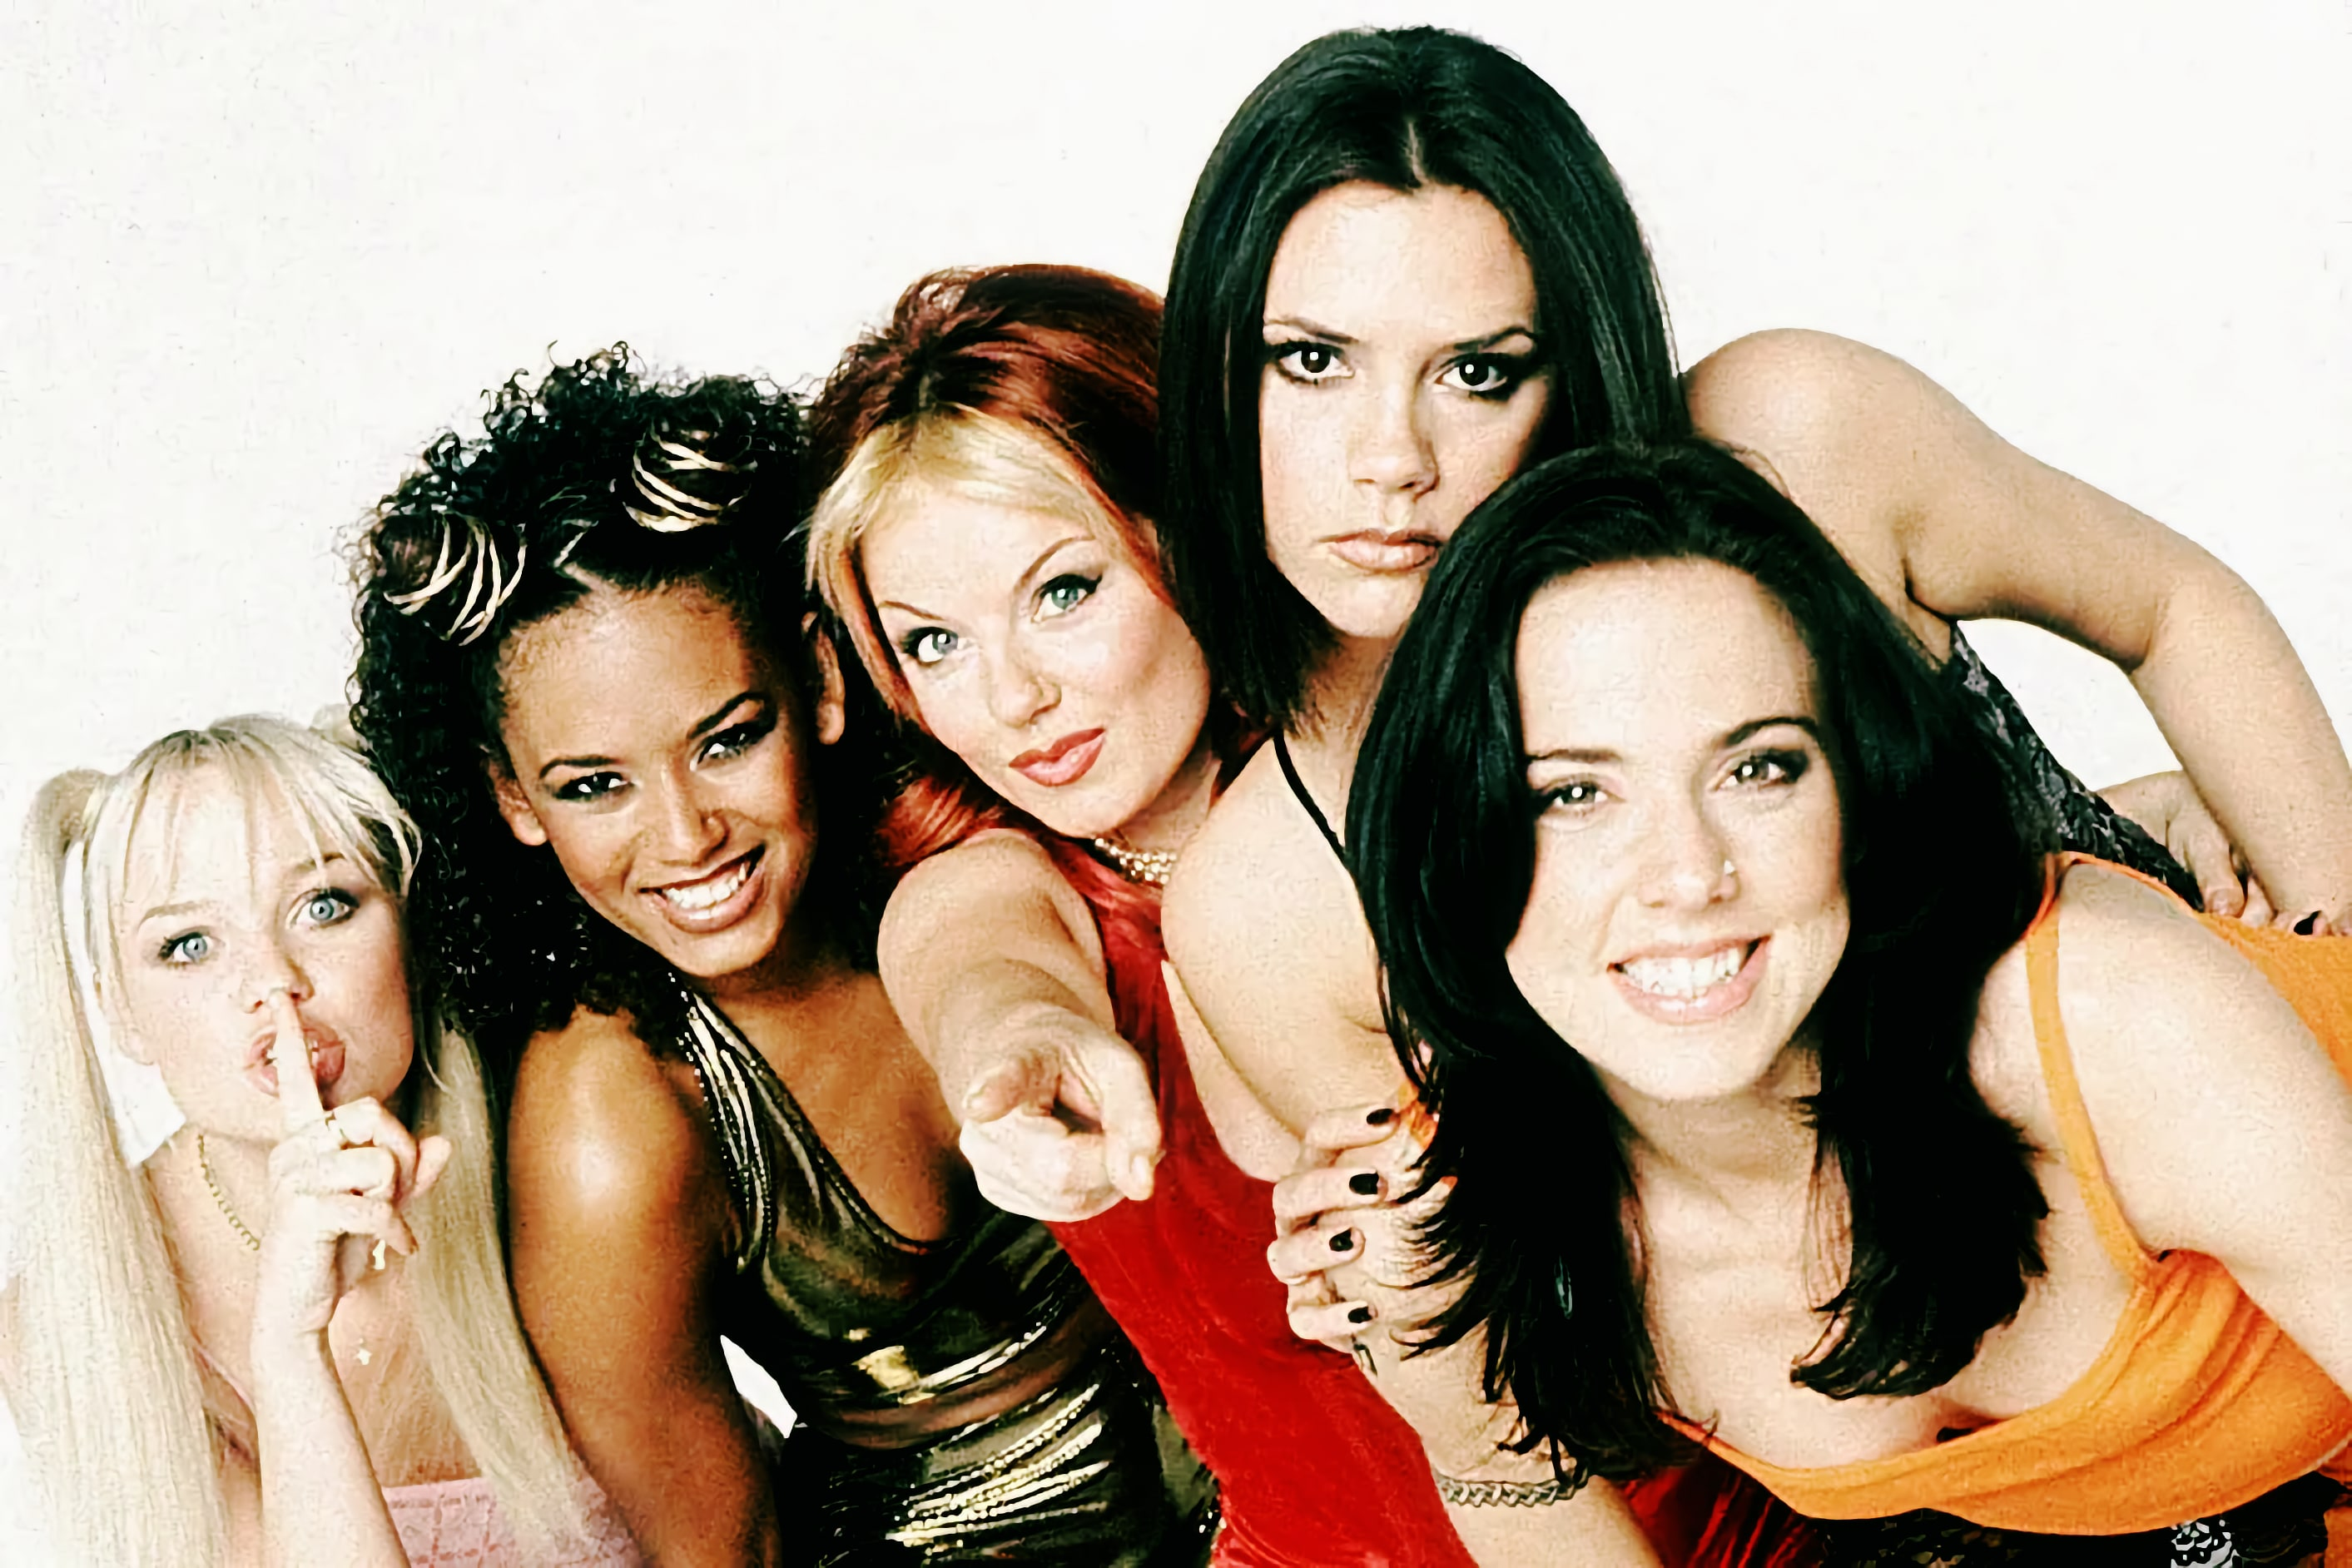
\includegraphics[height=5cm]{spice-girls-spice-world-billboard-1548.jpg}\\
\tiny{$^*$Wannabe by Spice Girls}
\end{frame}

% -----------------------------------------------
\begin{frame}{}
\begin{itemize}
    \item At first, it may seem that answers are the most important.
    \item The real goal is to learn how to \textbf{ASK questions}.
    \item When you can create thoughtful questions about a topic means you truly understand it.
\end{itemize}
\end{frame}

\end{document}